\chapter{既存手法}
本章では,既存手法であるgBoost\cite{gBoost}について説明する.
gBoostは線形計画問題で定式化されたブースティング手法であるLPBoost\cite{lpboost}と,
部分グラフの探索アルゴリズムを組み合わせたグラフの分類,回帰モデルである.
本研究ではグラフの分類問題を扱うため,以下では,問題設定,既存手法と順を追って説明する.

\section{グラフ分類問題}
まずはじめに,今回扱う問題であるグラフ分類問題について説明する.
グラフ分類問題とは,教師データとしてグラフとクラスラベルのペアの集合$\{G_n, y_n\}^{\ell}_{n=1}$を与えられた際,
未知のグラフデータに対するクラスラベルを予測する予測器$f$を学習する問題である.
扱うグラフは,連結であるものとする.
本研究では,クラスラベル$y$に関して,$(y \in \{+1, -1\})$となるような二値分類を対象として扱う.

\section{gBoost}
一般的に機械学習の線形モデルは,
扱う特徴に対してその線型結合の値を出力値として予測に用いる.
2値分類(+1 or -1)の場合,出力値の値が0以上の時に1,0未満の時に-1と予測する.
グラフ分類問題に用いる特徴量は様々なものが考えられるが,
gBoostではグラフデータに含まれる部分グラフの有無を特徴量として用いる.

入力として$\ell$個のグラフとクラスラベルのペアの集合
$\{G_n, y_n\}^{\ell}_{n=1} (y_n \in \{+1, -1\})$が与えられた時,
入力データに少なくとも1回は出現する全ての部分グラフを$\mathcal{T}$とする.
この時グラフ$G_n$は$|\mathcal{T}|$次元のベクトル$\bm{x}_n(x_{n,t} = \mathbb{I}(t \subseteq G_n), \forall t \in \mathcal{T})$として表現することができる.
$\mathbb{I}(\cdot)$は括弧内が真なら1,偽なら0を返す指示関数である.

この時,各特徴に対して仮説(hypothesis)と呼ばれる,弱学習器を以下で定義する.

\begin{equation*}
	h(\bm{x};t,\omega) = \omega (2x_t - 1).
\end{equation*}
$\omega \in \Omega = \{-1,1\}$はパラメータである.
この弱学習器を用いて,gBoostでは以下の線形分類モデルを構築する.
\begin{align}
	\label{eq:linear}
	f(\bm{x}) = \sum_{(t,\omega) \in \mathcal{T}\times \Omega} \alpha_{t,\omega} h(\bm{x};t,\omega).
\end{align}
$\alpha_{t,\omega}$は各弱学習器の重みであり,$\sum_{(t,\omega) \in \mathcal{T}\times \Omega} \alpha_{t,\omega}=1,\alpha_{t,\omega} \geq 0$を満たす.

gBoostでは,
LPBoostで定式化された以下の線形計画問題を主問題として解くことで,
式\eqref{eq:linear}の線形モデルの重み$\alpha_{t,\omega}$の値を導く.
\begin{align}
	&\min_{\bm{\alpha},\bm{\xi},\rho} -\rho + D \sum_{n=1}^{\ell} \xi_{i} \nonumber\\
	&\text{s.t.} \,\,\left\{
	\begin{aligned}
		&\sum_{(t,\omega) \in \mathcal{T} \times \Omega} y_{n} \alpha_{t,\omega} h(\bm{x_{n}};t,\omega) + \xi_{n} \geq \rho,
		\xi_{n} \geq 0,	n = 1, \dots , \ell,\nonumber \\
		&\sum_{(t,\omega) \in \mathcal{T} \times \Omega} \alpha_{t, \omega} = 1, \alpha_{t, \omega} \geq 0.
	\end{aligned}\right.
\end{align}
ここで,$\rho$はソフトマージン,$D=\frac{1}{\nu \ell}, \nu \in (0,1)$であり,$\ \nu\ $は誤分類に対するコスト制御のパラメータである.
一般に,変数$\bm{\alpha}$の数は部分グラフの総数であるため膨大であり,主問題を解くことは困難である.
したがって,主問題と等価な以下の双対問題を扱う.

\begin{align}
	\label{eq:dualprob}
	&\min_{\bm{\lambda},\gamma} \gamma \nonumber\\
	&\text{s.t.} \,\,\left\{
	\begin{aligned}
		& \sum_{n=1}^{\ell} \lambda_{n} y_{n} h(\bm{x}_{n};t,\omega) \leq \gamma,
		\forall(t,\omega) \in \mathcal{T} \times \Omega\\
		& \sum_{n=1}^{\ell} \lambda_{n} = 1, \,0 \leq \lambda_{n} \leq D, \,i = 1, \dots , \ell. 
	\end{aligned}\right. \end{align}

双対問題は,主問題に比べ制約式の数は多くなるが列生成法を用いることで解を得ることが可能となる.
列生成法は,制約なしの状態から始め,現制約を最も違反する制約を追加し,
最適化問題を解くという過程を繰り返すことで解を得る手法である.
最も違反する制約を見つける問題は以下の最大化問題と等価である.
\begin{equation*}
	(t^{*}, \omega^{*}) = \argmax_{t \in \mathcal{T} , \omega \in \Omega} \sum_{n=1}^{\ell} \lambda_{n}^{(k)} y_{n} h(\bm{x_{n}} ; t, \omega).
\end{equation*}
これに対して最大化する目的関数をgainと呼び以下の式で定義する.
\begin{align}
	\label{eq:gain}
	g(t, \omega) = \sum_{n=1}^{\ell} \lambda_{n}^{(k)} y_{n} h(\bm{x_{n}} ; t, \omega).
\end{align}
もし以下を満たすような弱学習器が存在しない場合,現在の解が双対問題の最適解となる.

\begin{equation*}
	\sum_{n=1}^{\ell} \lambda_{n}^{(k)} y_{n} h(\bm{x_{n}} ; t, \omega) > \gamma^{(k)}.
\end{equation*}

経験的に終了付近の制約追加による重みの更新は僅かであるため,
緩和項$\ \epsilon \ $を用いて以下のように終了条件を緩和することで,計算を効率化する.
\begin{equation*}
	\sum_{n=1}^{\ell} \lambda_{n}^{(k)} y_{n} h(\bm{x_{n}} ; t, \omega) > \gamma^{(k)} + \epsilon .
\end{equation*}
双対問題の終了条件緩和により得られる主問題の解は,$V^*$を緩和なしでの最適解とすると,$V \leq V^* + \epsilon$を満たす.\\

次にgBoostにおける特徴探索を考える.
特徴探索では重複無しに全部分グラフを列挙した探索空間であるDFSコード木\cite{gSpan} (図\ref{small_DFS})を用いる.
\begin{figure}[t]
	\centering
	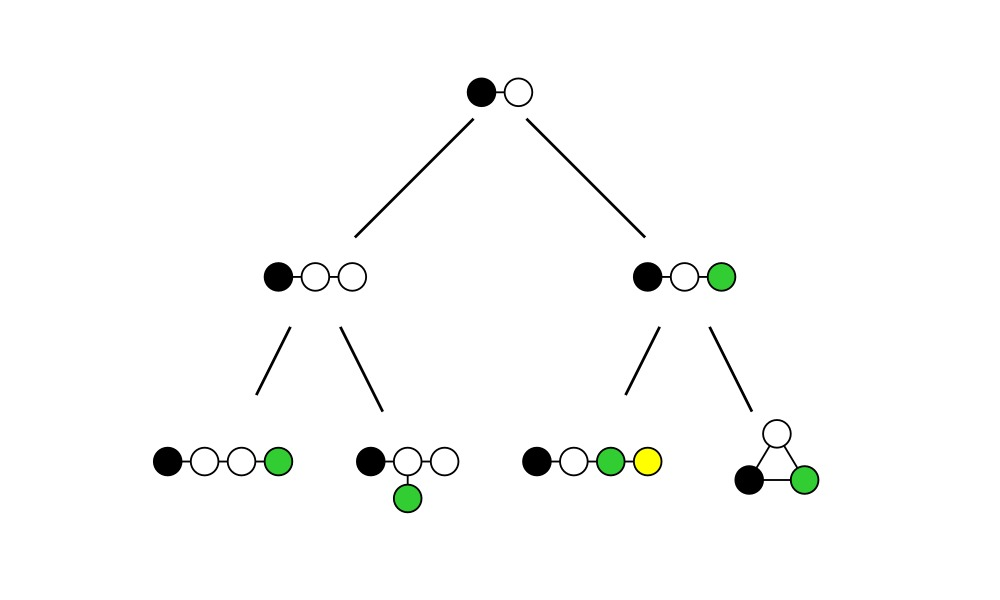
\includegraphics[width=70mm]{figure/small_DFS.jpg}
	\caption{DFSコード木}
	\label{small_DFS}
\end{figure}
DFSコード木は,全部分グラフをノードに含む他に,子が親の拡大グラフとなるという特徴を持つ.
この探索木を深さ優先順にたどり,各ノードにおいてgainを計算することで,最適な部分グラフを探索する.
一般に,部分グラフの総数は膨大となるため全てのノードを探索するためには相当なコストを要する.
しかし,子が親の拡大グラフとなる特徴を利用すると,
bound(子孫ノードでのgainの上限値)を計算することができるため,
安全な枝刈りを行うことが可能である.
boundの計算,枝刈り可能条件を以下に示す.

現探索部分グラフを$t$,その拡大グラフを$t'$とすると,
boundの値$b(t)$は以下の式で計算できる.
\begin{align}
	\label{eq:bound}
	b(t) = \max\{2 \sum_{\{n|y_{n}=+1, t \subseteq G_{n}\}} \lambda_{n}^{(k)} - \sum_{n=1}^{\ell} y_{n} \lambda_{n}^{(k)},	2 \sum_{\{n|y_{n}=-1, t \subseteq G_{n}\}} \lambda_{n}^{(k)} - \sum_{n=1}^{\ell} y_{n} \lambda_{n}^{(k)}\}.
\end{align}
枝刈り可能条件は,現探索までのgainの最大値を$g^{*}$とすると以下となる.
\begin{align}
	\label{eq:prune}
	g^{*} > b(t).
\end{align}
この枝刈りが有効に働くため,gBoostアルゴリズムは探索空間に対して効率よくモデルを構築することができる.
